\section{Diskussion}
    \subsection{Wheatstonesche Brückenschaltung}
    Für den Widerstand, der mit der Wheatstoneschen Brücke bestimmt wurde, ergibt sich ein Wert von $R_{13}=\qty{318,98(9,71)}{\ohm}$.
    Der tatsächliche Wert von Wert 13 wird hier als $R_{13}'$ definiert und beträgt $R_{13}'=\qty{319}{\ohm}$.
    Für den Quotienten von bestimmten Wert und Realwert gilt $\frac{R_{13}}{R_{13}'}=0,9999373\pm0,0304389$.

    \noindent Für Wert 11 ergibt sich mit $R_{11}=\qty{490(15)}{\ohm}$ und $R_{11}'=\qty{489,9}{\ohm}$ $\frac{R_{11}}{R_11'}=1,002\pm0,031$.

    \subsection{Kapazitätsmessbrücke}
    Der, mit der Kapazitätsmessbrücke bestimmte Widerstand, hat den Wert $R_8=\qty{690(21)}{\ohm}$.
    Die hier bestimmte Kapazität $C_8=\qty{361(11)}{\nano\farad}$. 
    Die realen Werte sind $R_8'=\qty{564}{\ohm}$ und $C_8'=\qty{294,1}{\nano\farad}$.
    Die damit gebildeten Quotienten sind $\frac{R_8}{R_8'}=1,223\pm0,037$ und $\frac{C_8}{C_8'}=1,227\pm0,037$.
    Bei Wert 9 sind die gemessenen Werte $R_9=\qty{488(15)}{\ohm}$ und $C_9=\qty{511(7)}{\nano\farad}$.
    Für die tatsächlichen Werte gilt $R_9'=\qty{464,9}{\ohm}$ und $C_9=\qty{433,71}{\nano\farad}$.
    Damit sind die Verhältnisse $\frac{R_9}{R_9'}=1,05\pm0,03$ und $\frac{C_9}{C_9'}=1,178\pm0,016$.
    
    \subsection{Induktivitätsmessbrücke}
    Bei der Induktivitätsmessbrücke wurde mit Realwerten von $R_{18}'=\qty{360,5}{\ohm}$ und $L_{18}'=\qty{48,82}{\milli\henry}$ und den gemessenen Werten ebenfalls die Quotienten berechnet.
    Die eingesetzten gemessen Werte sind dabei $R_{18}=\qty{412(13)}{\ohm}$ und $L_{18}=\qty{34,16(1,04)}{\milli\henry}$.
    Es ergibt sich $\frac{R_{18}}{R_{18}'}=1,143\pm0,036$ und $\frac{L_{18}}{L_{18}'}=0,6997\pm0,0213$.

    \subsection{Maxwellsche Messbrücke}
    Der hier ausgerechnete Widerstand beträgt $R_18=\qty{366.687(11.130)}{\ohm}$ und die Induktivität $L_18=\qty{55.278(2.872)}{\milli\henry}$.
    Verglichen mit den Bereits oben genannten Angaben für Wert 18 ergibt sich, dass $\frac{R_{18}}{R_{18}'}=1.02\pm0.03$ ist und
    $\frac{L_{18}}{L_{18}'}=1.132\pm0.029$. Es ist erkenntlich, dass die Maxwellsche Messbrücke Messwerte liefert, die näher am angegebenen
    Wert liegen, als die Induktive bei einem ähnlichen Fehler.

    \subsection{Fazit}
    Im Gegensatz zu den anderen Methoden ist mit der Wheatstoneschen Brückenschaltung die genauste Bestimmung des Widerstandes gelungen.
    Das könnte daran liegen, dass in den anderen Aufbauten Kondensatoren und Spulen verbaut sind. 
    Diese werden hier nämlich als widerstandslos angenommen, jedoch sind perfekte Kondensatoren und Spulen nicht zu realisieren.
    Das könnte der Grund für die Größeren Abweichungen bei den anderen Methoden sein.

    \subsection{Klirrfaktor}
    Der Klirrfaktor $k=0.87$ zeigt hier das Verhältis zwischen den Amplituden der Grundschwingung und der zweiten Oberschwingung,
    da nur die zweite betrachtet wird.
    Entsprechend gilt dann, dass die Amplitude von $U_2$ $\qty{87}{\percent}$ von $U_1$ beträgt.

    \begin{figure}
        \centering
        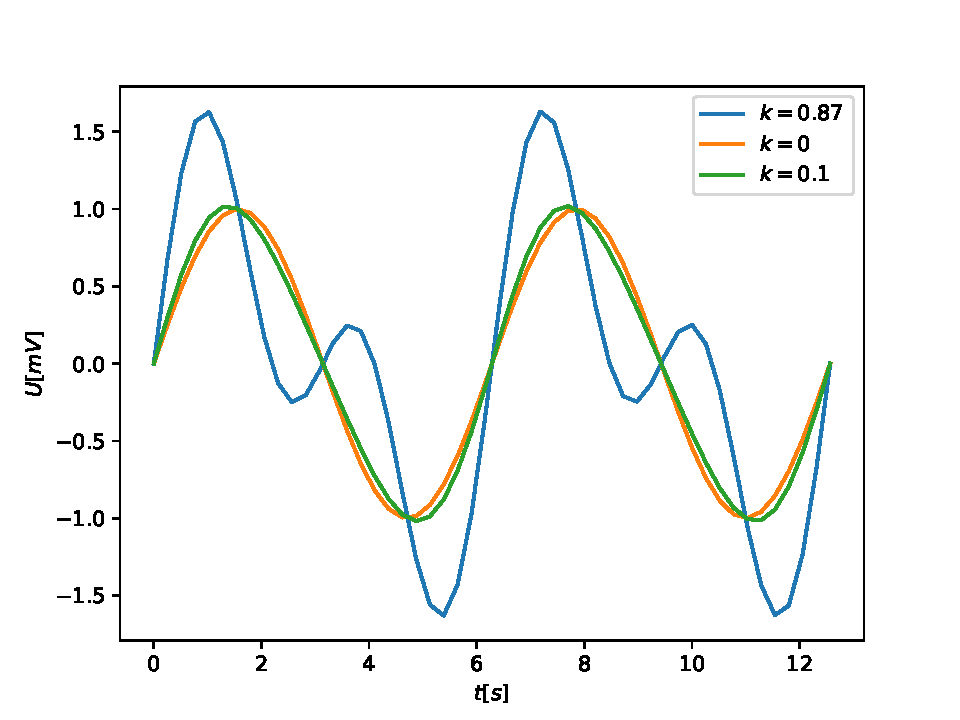
\includegraphics{./Klirr_Model.pdf}
        \caption{Modellierung von Sinusschwingungen für unterschiedliche Werte von k}
        \label{fig:klirr_mod}
    \end{figure}

    \noindent Wie \ref{fig:klirr_mod} modellhaft zeigt, hat ein solch großer Wert von $k$ einen signifikanten Einfluss auf den Spannungsverlauf, einen
    Verlauf, der auf dem Oszilloskop so nicht sichtbar war.
    Allerdings wurden für die berechnung von k störende Frequenzen höherer Ordnung vernachlässigt, was den Wert von $k$ weiter
    verändern würde und die obige einfache Beziehung zwischen $U_2$ und $U_1$ ermöglichte. Desweiteren ist es möglich, dass 
    das Spannungsminimum nicht bei $\qty{150}{Hz}$ liegt, da die Frequenz nur in groben Schritten gemessen wurde verglichen mit einer
    größeren Steigung in diesem Frequenzintervall, wie in \ref{fig:frequenzverhältnis} dargestellt ist. Der theoretische Wert von
    $f_0$, welcher über die Eigenfrequenz über \ref{eqn:omega} berechenbar ist, beträgt $\qty{160.27(6.80)}{\hertz}$, was nahelegen würde,
    dass $f_0$ größer ist, als der aus \ref{frequenzen} genommene Wert. Entsprechend ist es wahrscheinlich, dass diese Ungenauigkeiten $k$ größer
    werden lassen haben, als er eigentlich ist, oder das Vernachlässigen der höheren Frequenzen das Spannungsbild zu stark verändert hat.

    \label{sec:Diskussion}
